% Figure: DeltaSort worst-case movement diagram
\begin{figure}[h]
\centering
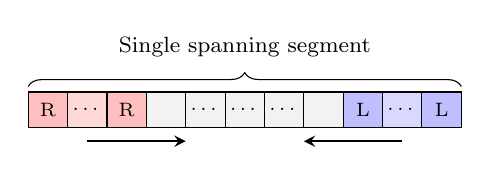
\begin{tikzpicture}[
    cell/.style={minimum width=0.5cm, minimum height=0.45cm, draw, font=\scriptsize, inner sep=0pt, outer sep=0pt, anchor=center},
    right/.style={cell, fill=red!25},
    left/.style={cell, fill=blue!25},
    clean/.style={cell, fill=gray!10, font=\scriptsize},
    segbrace/.style={decorate, decoration={brace, amplitude=5pt}},
    seglabel/.style={font=\footnotesize},
]

\def\yarr{0}
\def\cellw{0.5}

% Place cells at exact positions (center anchored, spaced by cellw)
\node[right] (c0) at (0*\cellw, \yarr) {R};
\node[cell, fill=red!15] (c1) at (1*\cellw, \yarr) {\dots};
\node[right] (c2) at (2*\cellw, \yarr) {R};
\node[clean] (c3) at (3*\cellw, \yarr) {};
\node[cell, fill=gray!10] (c4) at (4*\cellw, \yarr) {\dots};
\node[cell, fill=gray!10] (c5) at (5*\cellw, \yarr) {\dots};
\node[cell, fill=gray!10] (c6) at (6*\cellw, \yarr) {\dots};
\node[clean] (c7) at (7*\cellw, \yarr) {};
\node[left] (c8) at (8*\cellw, \yarr) {L};
\node[cell, fill=blue!15] (c9) at (9*\cellw, \yarr) {\dots};
\node[left] (c10) at (10*\cellw, \yarr) {L};

% Brace spanning entire array
\draw[segbrace] ([yshift=2pt]c0.north west) -- ([yshift=2pt]c10.north east);
\node[seglabel] at (5*\cellw, 0.8) {Single spanning segment};

% Arrows below showing movement directions
\draw[->, thick, >=stealth] (1*\cellw, -0.4) -- (3.5*\cellw, -0.4);
\draw[->, thick, >=stealth] (9*\cellw, -0.4) -- (6.5*\cellw, -0.4);

\end{tikzpicture}
\caption{Worst-case configuration for DeltaSort is formed when updated values cluster at ends of the array and form a single spanning segment.}
\label{fig:worst-case}
\end{figure}
